
\section{COMPUTATIONAL READINESS}  

%% Proposals will be assessed on the need for, readiness to use, and
%% reasonableness of the request for resources. {\bf This section is
%%   typically about 5 pages.}

The proposed work uses a suite of simulation codes.  \maestro\ is a
low Mach number hydrodynamics code suited to convective flows; \castro
is a compressible radiation-hydrodynamics code designed for high Mach
number flows.  These two codes share a common framework, built around
the \boxlib\ library.  We note that both of these codes are freely
available to the community and any improvements to their parallel
performance based on the work proposed here will benefit all users of
the codes.  A small set of calculations (explosive models of sub-Ch)
will use \flash, a compressible hydrodynamics code, as these
calculations are already implemented with \flash.  Finally, the
core-collapse simulation proposed here will use \chimera, a
compressible hydrodynamics code with ray-by-ray neutrino transport.
The unique features of titan, in particular the GPUs on each node, are
of critical importance to meeting the science goals proposed
here---GPUs, will allow us to consider bigger networks.  We have
microphysics code running on the titan GPUs already, and discuss our plans
for furthering our performance below.


\subsection{Use of Resources Requested}

%% Describe your proposed production simulations and state how the runs
%% are tied to each of your project's goals and milestones (the Milestone
%% Table). For the simulations you plan to carry out during production
%% runs, provide a
%% \begin{enumerate}
%% \item description of what jobs are going to be run and how they relate
%%   to the research/development objectives given above;
%% \item description of processor/core use for large runs (e.g.,
%%   10,000-hour run with 100 cores, or ten 10-hour runs with 10,000
%%   cores, for a 1,000,000-hour allocation);
%% \item clear, detailed explanation as to how you calculated the
%%   requested number of processor hours; and
%% \item summary of your anticipated annual burn rate (e.g., linear or
%%   with periods of peak usage).
%% \end{enumerate}
%% \vspace{-.2in}

Our list of large jobs to run along with detailed time estimates is
given in the previous section.  In each case, the time estimates were
computed based on actual runs of the proposed problem on titan---these
problems are already running there.  The convection jobs all share
something in common---the need for long time-integration.  This means
{\em many} trips through the queue (it's not uncommon to require 500
wallclock hours, broken up into may smaller segments).  With 10,000
cores, this is 5~Mh---a number representative of many of our jobs.
This will represent the typical job size for the base calculations.
The addition of bigger networks will push the base calculations up to
larger core counts in subsequent years.

There are several large calculations each year when that will need more
processors.  The biggest XRB runs will require 10,000s of cores.  We
scale well to that point now, and planned developments described
below will make this a more typical size.  For the WDWD simulations,
as the stars merge, the number of AMR grids created will dramatically
rise, as a result, the last 10\% of the simulation may require
10$\times$ more processors.  The same will be true of the
\castro\ continuation of our \maestro\ sub-Ch model.

Our usage throughout the year will have periods of intense
usage---when we have decided on our initial conditions and are running
a suite of calculations for a paper.  Many of us teach, and will be
less active during the semester, but the graduate students will be running
steadily throughout the year.


\paragraph{Leadership Classification: }
%
The job characteristics as described above are hundreds of hours on
10k cores for our standard jobs and several 10,000s of cores (again
for hundreds of hours) for our biggest jobs.  We are proposing 10s of
jobs per year, with an average cost of a few Mh, and the biggest jobs
requiring 25 Mh.  These numbers cannot be met by any facility other
than through INCITE.  We can run at this scale today.  Any larger, and
it becomes difficult to get the runtime needed to complete our jobs.
Our largest jobs will be on the leadership class by themselves,
requiring $\sim 20$\% of the machine, and our wide range of concurrent
moderately-sized studies for the proposed simulations will utilize
more than 20\% of the total machine.  Finally, we have been investing
our time in porting our microphysics to the GPUs.  This is essential
to implementing the physics we require.  We have worked in close
collaboration with the staff at OLCF to get our codes running with
OpenACC.  A the moment, our microphysics solvers achieve atleast
parity on the GPUs when compared to full-node performance with OpenMP,
and in some cases, are sped up by a factor of a few.  For this
investment to payoff, we need a machine with GPUs on all of the
nodes---titan has been our target.  Only INCITE resources meet these
needs.

%% Summarize the requirement that best exemplifies the proposed
%% computational work. Leadership targets in the INCITE program typically
%% include one or both of the following categories:

%% \begin{enumerate}
%% \item Use of 20 percent or more of the system for production
%%   simulations. Parameter sweeps, ensembles, design of experiments, and
%%   other statistical methods that require large numbers of discrete or
%%   loosely coupled simulations may be considered capability-class
%%   campaigns. See the FAQS <link> for details and qualifiers.
%% \item Specific architectural needs that can only be met by the LCF.
%% \end{enumerate}

%% 20 \% of titan is currently about 3738 nodes (59,808 cores + GPUs)...


\subsection{Computational Approach}

%% Provide a detailed description of your computational approach,
%% including a discussion of the state of the art in the field. The
%% description should also mention:

%% \begin{enumerate}
%% \item Particular libraries required by the production and analysis
%%   software, algorithms and numerical techniques employed (e.g., finite
%%   element, iterative solver), programming languages, and other
%%   software used.
%% \item Parallel programming model(s) used (e.g., MPI, OpenMP, Pthreads,
%%   CUDA, OpenACC).
%% \item Project workflow including the role of analysis and
%%   visualization; identify where the analysis will be done and any
%%   potential bottlenecks in the analysis process.
%% \item Software workflow solution (e.g., pre- and postprocessing
%%   scripts that automate run management and analysis) to facilitate
%%   this volume of work.
%% \item I/O requirements (e.g., amount, size, bandwidth) for restart,
%%   analysis, and workflow. Highlight any exceptional I/O needs.
%% \item Data storage requirements. Estimate anticipated cumulative size
%%   of stored data at the end of the requested award. What do you plan
%%   to do with the data at the end of the project? Do you plan to share
%%   the data or make it public? Do you have tools and/or plans to reduce
%%   the data? Justify data storage needs that exceed 1 petabyte.
%% \end{enumerate}

\paragraph{\maestro\ and \castro: } 
%
\maestro\ decomposes the fluid state into a 1D radial hydrostatic base
state and a perturbational Cartesian state.  A divergence constraint
on the velocity field captures the compressibility due to background
stratification and local heating/diffusion sources.  The resulting
system allows for much larger time steps to be taken compared to
corresponding compressible codes ($\sim 1/M$ larger), where $M$ is the
Mach number.  The algorithm \cite{multilevel} utilizes a second-order
accurate approximate projection method, developed first for
incompressible flows.  Fluid quantities are advected using an unsplit
Godunov method, with reactions incorporated via operator splitting.
The provisional velocities are then projected onto the space that
satisfies the divergence constraint.  The projections involve elliptic
solves, solving a variable-coefficient Poisson problem, computed using
a multigrid algorithm.  AMR is used to achieve high spatial
resolution.  \maestro\ is written primarily in Fortran 95 and is
parallelized using MPI and OpenMP.  It is highly portable, and
regularly runs at the OLCF, NERSC, and NCSA.

\castro~\cite{castro} is based on a compressible flow formulation in
Eulerian coordinates and includes self-gravity and reaction networks.
All \castro\ calculations will use AMR on a 3D Cartesian grid.  The
hydrodynamics in \castro\ is based on the piecewise parabolic method
(PPM)~\cite{ppmunsplit} and is designed to work with a general convex
equation of state.  \castro\ supports Newtonian self-gravitational
forces through either a simple monopole approximation or a full
solution of the Poisson equation using geometric multigrid techniques.
Radiation is incorporated into \castro\ using flux-limited diffusion,
either in a gray approximation or multigroup.  The approach to AMR in
\castro\ uses a nested hierarchy of logically-rectangular grids with
simultaneous refinement of the grids in both space and time.  The
integration algorithm on the grid hierarchy is a recursive procedure
in which coarse grids are advanced in time, fine grids are advanced
multiple steps to reach the same time as the coarse grids and the data
at different levels are then synchronized.  The synchronization for
self-gravity is similar to the algorithm introduced by
\cite{miniati-colella}.

Both \maestro\ and \castro\ uses a hybrid programming model based on
MPI and OpenMP.  For \castro, OpenMP uses tiling to efficiently scale
to many-core architectures.  \MarginPar{tiling ref?}  Distribution of
grid patches to nodes using MPI provides a natural coarse-grained
approach to distributing the computational work, while threading of
loops over zones in a grid using OpenMP provides effective
fine-grained parallelization.  Both codes use the same interface to
the EOS and thermonuclear reaction networks.  This enables us to
switch from a low Mach number simulation with \maestro\ to a fully
compressible simulation using \castro\ without changing the underlying
physics.

For analysis, \maestro\ and \castro\ dump out global diagnostics at
each time step and plotfiles at regular intervals.  The visualization
packages \visit\ and \yt\ have native support for the \boxlib\ file
format.  We expect the largest simulations to output about 100--200 TB
each in plotfiles, putting the storage needs at about 800 TB in year
1, rising to 1 PB in year 3.  We will save plotfiles for as long as
needed to finish the analysis and publication of the results.  Only a
minimal set of checkpoint files will be archived.  Where possible, we
will store output in single precision to conserve space.

\paragraph{\flash: }

\paragraph{\chimera: }


\subsection{Parallel Performance}

%% Provide direct evidence, {\bf including supporting quantitative data},
%% for your production application's parallel performance for the
%% intended research simulations. Ideally, the proposing team will have
%% generated the data. If you cite work by others, explain why it is
%% applicable here. You should use the application code you intend for
%% the production work, not a related code. Data for sample systems not
%% related to the intended research is undesirable. Performance
%% benchmarking should reflect all I/O requirements. Parallel performance
%% data in either strong or weak scaling mode must be provided. Explain
%% how the strong or weak scaling applies to the proposed work. See the
%% examples at the end of this document.

\begin{figure}[t]
\centering
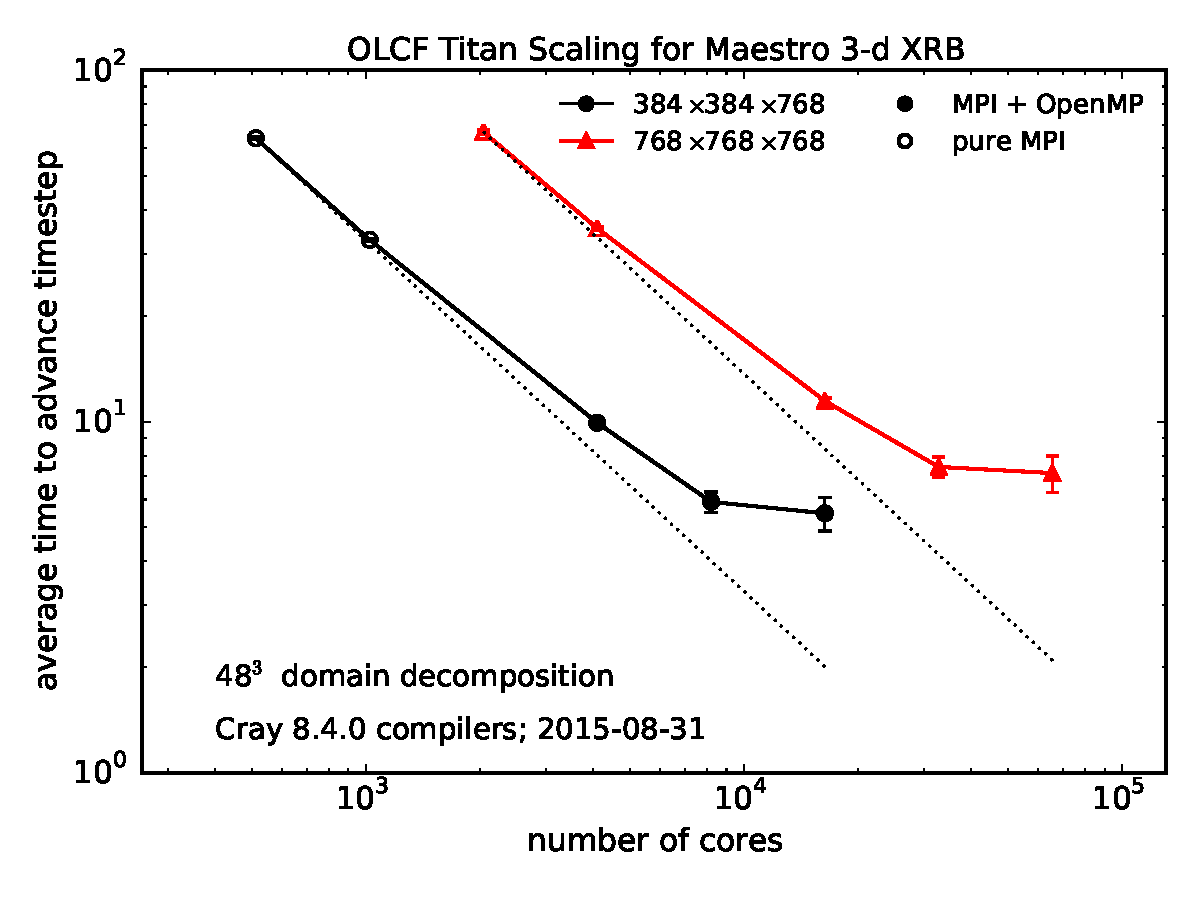
\includegraphics[width=0.49\linewidth]{titan_xrb_scaling}
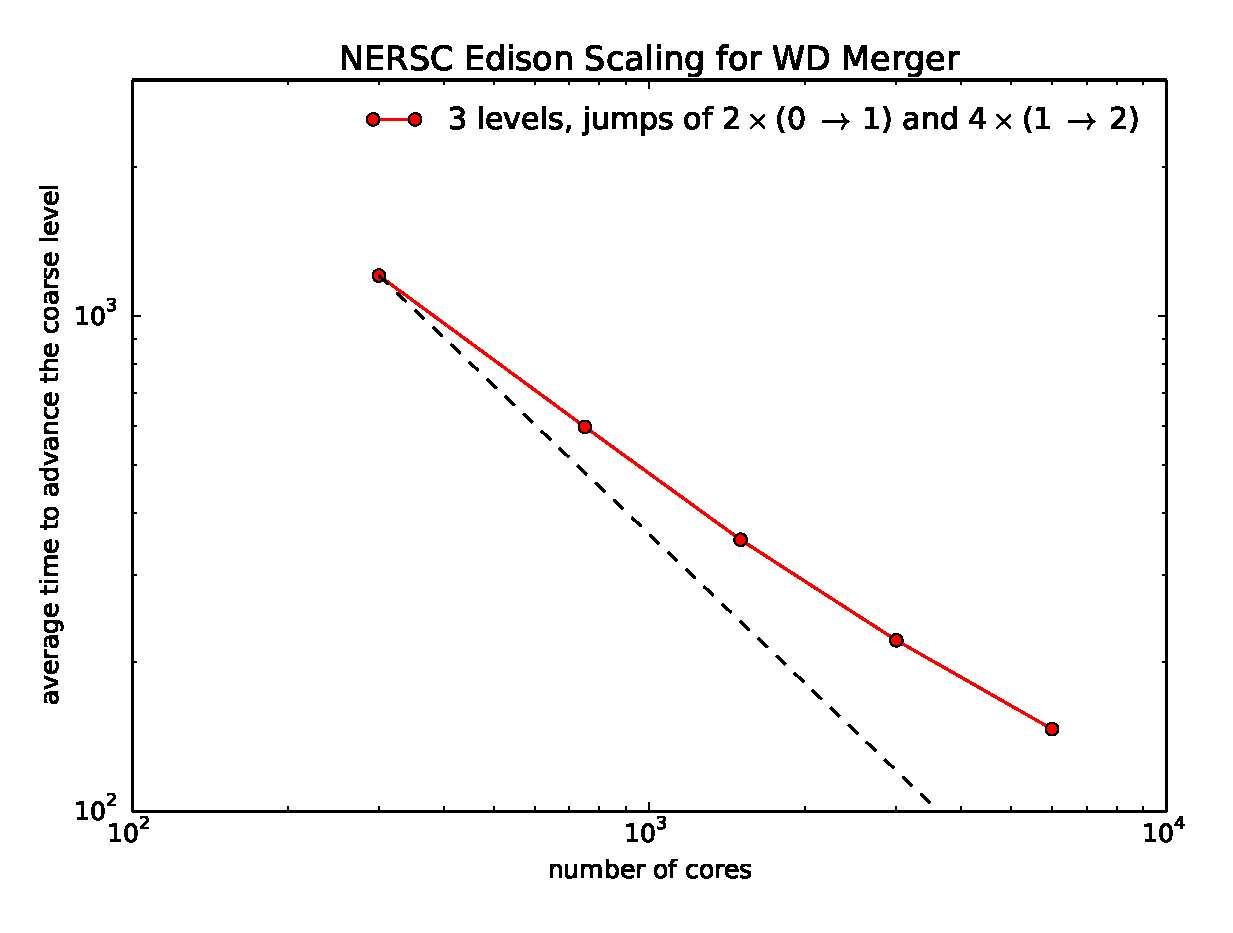
\includegraphics[width=0.49\linewidth]{edison-wdmerger-scaling.eps} \\
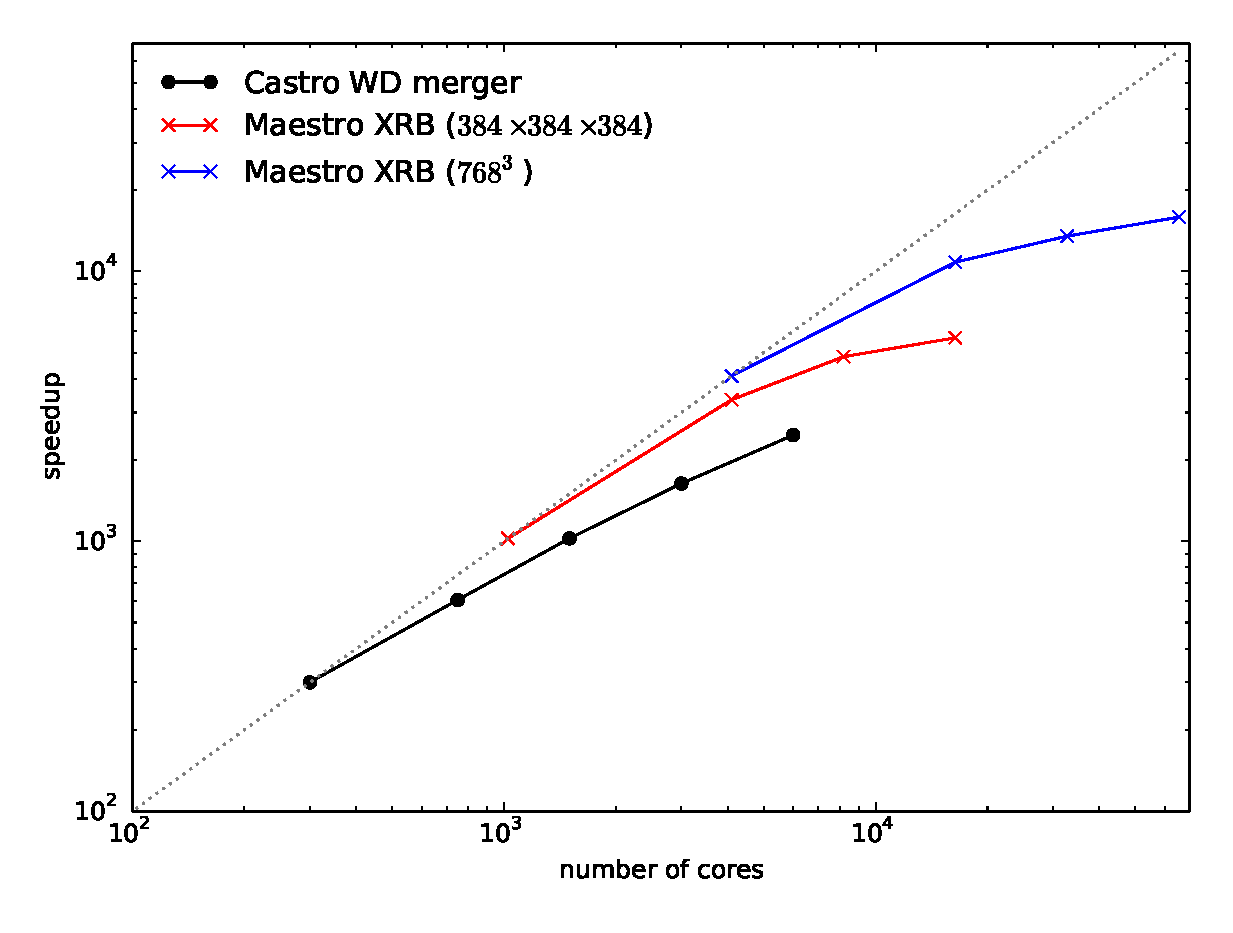
\includegraphics[width=0.4\linewidth]{speedup}
\begin{minipage}[b]{0.55\linewidth}
\caption{\label{fig:scaling} (top left) \maestro\ XRB strong
  scaling---two problem sizes are shown.  In each case, the time to
  advance the solution is the average of 10 steps.  Comparing the two
  problem sizes shows the weak scaling.  The turn-up at the highest
  core count for each problem size is NUMA-related---going from 1 MPI
  task per socket to 1 MPI task per node (top right) \castro\ strong
  scaling for the initial WDWD problem,
  run on the NERSC Edison machine.  This solves the full Poisson
  problem using multigrid with isolated boundary conditions. (left)
  Speed-up plot for the \maestro\ and \castro\ strong scaling data.}
\end{minipage}
\end{figure}


%% In year 1, the majority of our jobs will use \maestro, so we focused in
%% detail in obtaining real-world scaling numbers on titan for the main
%% year 1 jobs.

\paragraph{\maestro: }
%
Figure~\ref{fig:scaling} shows the strong scaling behavior for our
\maestro\ XRB problem on titan.  A subset of this same information is
shown in a speedup plot as well (Figure~\ref{fig:speedup}).
For \MarginPar{need to update speedup} \maestro\ strong scaling, we
explored two problem sizes (a 3D XRB with a domain of
384$\times$384$\times$768 zones, and one that is twice as wide in each
lateral direction, $768^3$).  We always assigned one grid per MPI task
and experimented with 1, 4, 8, or 16 OpenMP threads per MPI task.  We
see that we get good strong scaling over a decade increase in
processor count.  Note, we did not explore assigning tasks to specific
NUMA nodes in this test.  Finally, it seems that using 16 threads
incurs a slight performance penalty over lower thread counts.  The
bigger job has $4\times$ as much work and is run on $4\times$ the
number of processors as the corresponding smaller job.  Looking at the
first point in the curve and comparing to the corresponding point in
the smaller-job-size curve, we see that we have excellent weak scaling
as we increase the job size.  The strong scaling curve for this larger
problem shows that \maestro\ is reaching up to effective use of 20\%
of the machine.  Oue largest XRB runs will be atleast as large as the
large domain studied here.


The low Mach number constraint in imposed through a divergence
constraint on the velocity field.
\maestro\ uses two different multigrid solvers in the algorithm to
enforce this constraint.  At
the half-time, a cell-centered multigrid solver enforces the low Mach
divergence constraint on the velocities that go into the fluxes.  At
the final time, a node-centered (nodal) multigrid solver enforces
this constraint on the final velocity field.
Finer-grained timers tell us that the main scaling bottleneck is in
the nodal multigrid solver.  We have a plan to improve this scaling
that we expect to implement in the near future---we discuss it 
in section 3.5 below.  We note that this test corresponds to the 
proposed XRB simulations, which will run in exactly the fashion
tested here.  The sub-Ch and URCA \maestro\ simulations will exercise the
same parts of \maestro\ and we would expect similar scaling.  For
both problems, our plans have us increasing the reaction network in
later years---this will only improve scaling since the network is purely
local physics.

\paragraph{\castro: }
%
 For \castro, Figure~\ref{fig:scaling} (top-right) shows a  \MarginPar{Mike and Max will update}
weak scaling study where we put a WD on the adaptive grid and
simulated hydrodynamics with self-gravity using a monopole
approximation---this is representative of the sub-Ch
\castro\ simulations proposed.  This was run on the pre-titan hardware
(jaguarpf).  We considered both a single level and a two-level case
where the coarse resolution is equivalent to the single level case.
Both scale well to approximately 200K processors.  We note that the
2-level case does approximately three times the work of the single
level case.  The data shows an overhead of approximately 15-20\% for
AMR; however, achieving the same resolution as the two-level
simulation with a uniform grid would be a factor of 16 more than the
single level example treated here.

Our scaling numbers for the WDWD problem consider the initial stage,
when the stars are not yet interacting.  This is shown in the bottom
left panel of Figure~\ref{fig:scaling} and in the speedup plot, Figure~\ref{fig:speedup}.
The calculations were run on the NERSC Edison
platform, a Cray machine that shares many characteristics with titan.
This problem uses 3 levels in the grid hierarchy, level 0 is $480^3$,
level 1 is $2\times$ finer than level 0, and level 2 is $4\times$
finer than level 1, giving us an effective grid of $3840^3$.  This is
typical of the size problem we will want to run.  Gravity is done
using a full Poisson solve with multigrid, with the isolated boundary
conditions constructed by doing a multipole expansion (up to $l=6$) on
the coarsest grid.  \castro\ and \maestro\ share the same
cell-centered multigrid solver from \boxlib, and our early numbers
show that the gravity solve with isolated boundary conditions takes
approximately 25\% of the runtime for a WDWD problem where the stars
have not yet begun interacting.  We scale for over a decade in core count.  At high core counts, we become work
starved---there are too few grids at the fine level to redistribute equally.  As the stars interact, many more grids will be created
(about an order-of-magnitude increase is expected), and this will
improve the scaling and allow us to move to higher core counts.  Our
plan is therefore to start this problem on a moderate number of cores
and move to larger core counts as it evolves.  The addition of burning
in year 2 will greatly increase the local physics, further improving
the scaling.

\paragraph{\flash: } \MarginPar{Tom---do you have \#s specific to your problem?}

\paragraph{\chimera: } \MarginPar{Bronson}

\paragraph{I/O: } 
%
We directly measured the time to output from
\maestro\ on titan, writing a 50~GB plotfile at a data rate
ranging from 4--12 GB/s.  We note that I/O takes less than 1\% of our
runtime, and it will not be an issue for the proposed runs.
As \castro\ uses a similar I/O strategy, we expect it to attain the
same performance.    \chimera\ uses a custom, tunable, multi-file, parallel HDF I/O module to 
acheive I/O performance that takes no more than 2\% of runtime at 131000 cores on Titan. The \flash\ I/O benchmark (derived directly from the 
ORNL version of the code) is a standard benchmark in the OLCF testing harness, which is run intermittently to ensure performance of the
Atlas file system at OLCF.  All of our codes have checkpoint/restart capability 
to make effective use of titan's queue system.



\subsection{Developmental Work}

\MarginPar{need Tom, Adam, and Max to discuss GPU microphysics, Max for GPU hydro, Weiqun for tiling}

Both \maestro\ and \castro\ already scale well on titan and are
capable of running the proposed science.  Nevertheless, we are
continually working on the performance of these codes, and in
particular, in the last year have been actively targeting titan and
its GPUs.  Our graduate students have been the lead on this effort.

As part of our ongoing CAAR project, we recently added the capability
to evolve nuclear reaction networks of arbitrary sizes into the FLASH
code. It is important to note, however, that the computational expense
to evolve such reaction networks increases as (at least) the number of
species squared. In order to ameliorate part of this increased
expense, we added OpenMP threading (within blocks) to the burning
module. Figure \ref{fig:speedup_flash} shows $\sim$8$\times$ speedup
when using this OpenMP version of the burner with 16 threads (relative
to no threading) and an additional 2$\times$ speedup from improved
load balancing. We also developed a version of the burner that targets
the GPUs on Titan through the use of batch cuBLAS library routines in
addition to OpenMP threading. This figure also
shows a comparison of the two versions of the burning module, where
the GPU-enhanced version shows an additional 20-30\% speedup relative
to the OpenMP version at most epochs of the simulation. Relative to no
threading, this gives a total speedup of $\sim$18$\times$.


\begin{figure}[t]
\centering
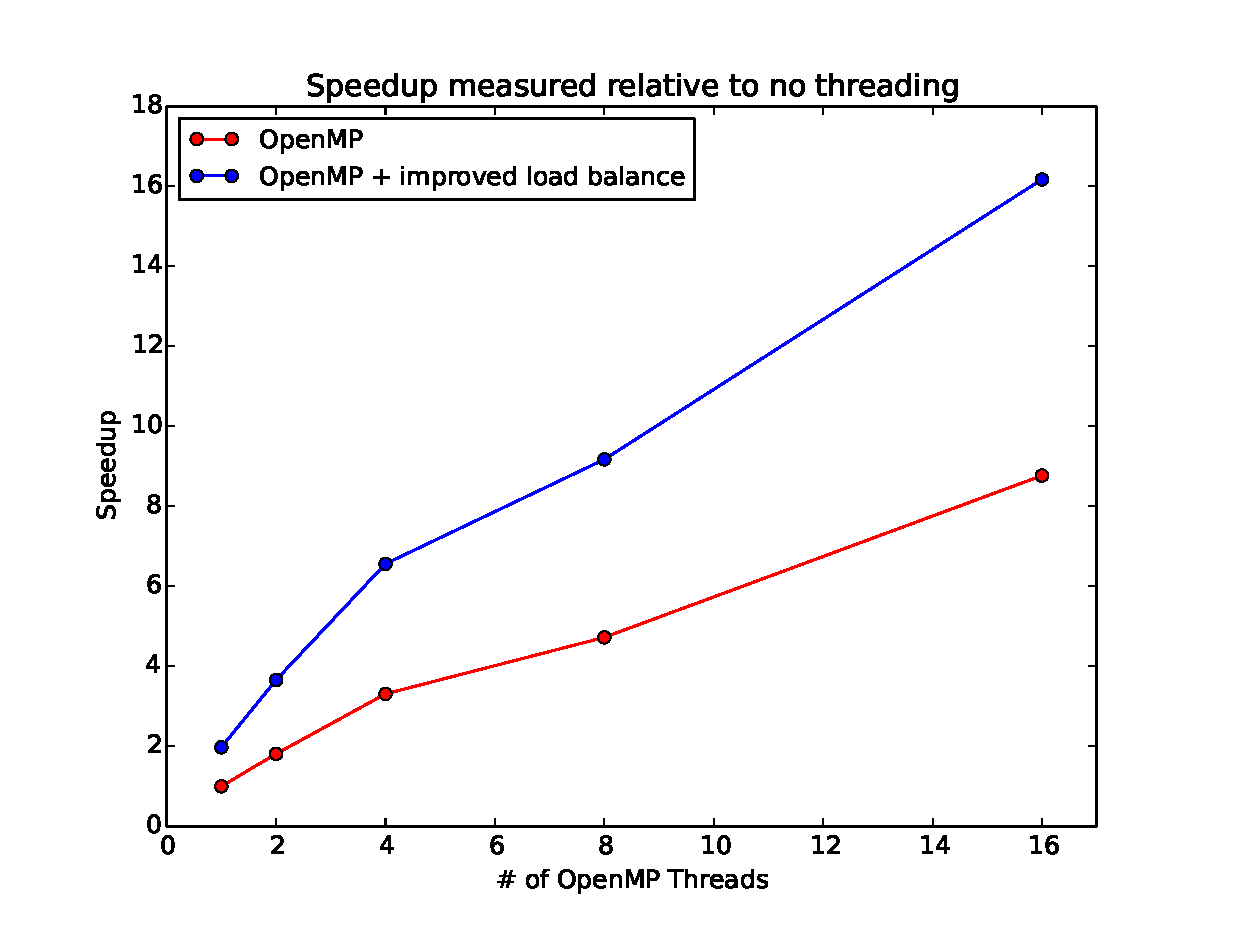
\includegraphics[width=0.48\linewidth]{speedup_OpenMP.eps}
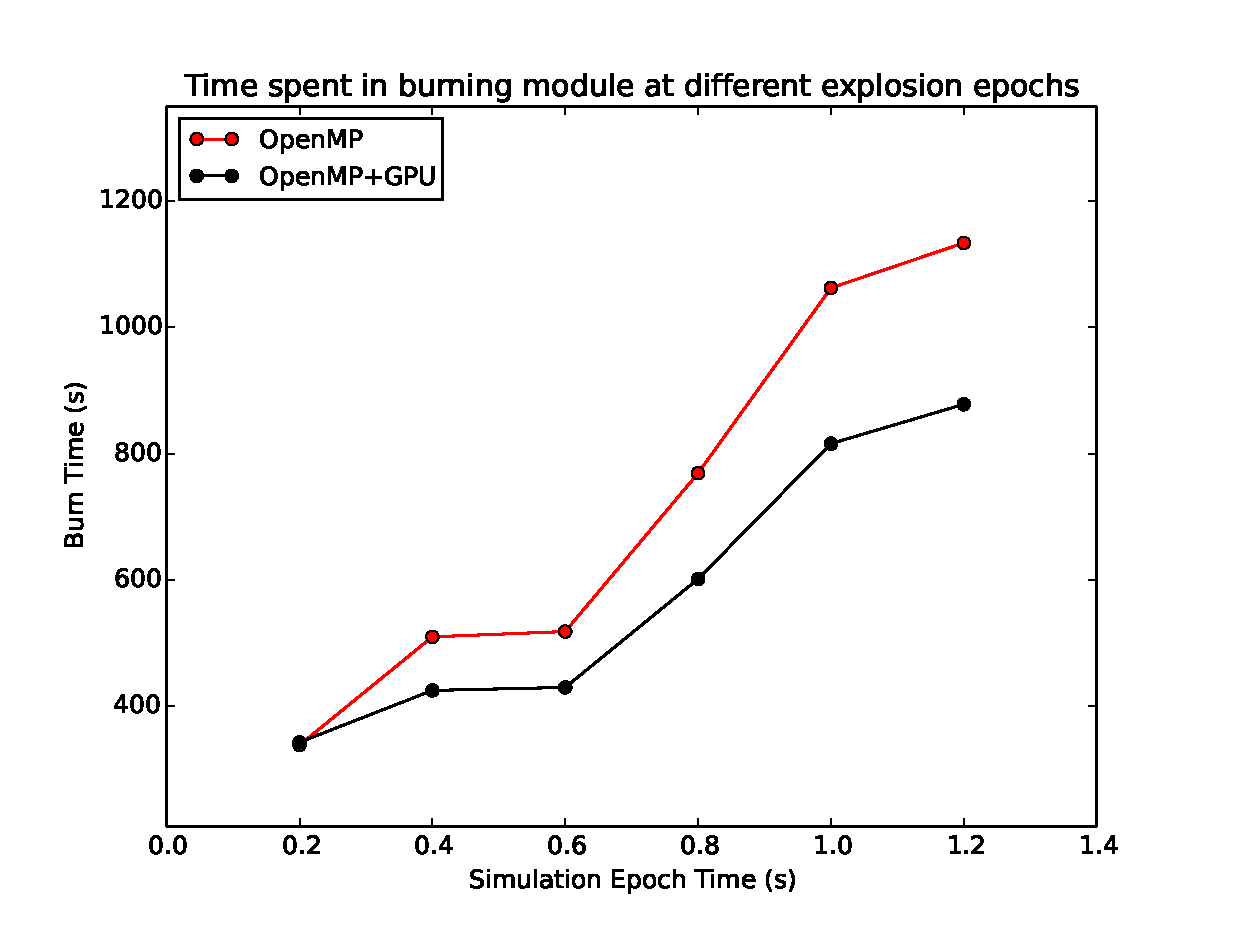
\includegraphics[width=0.48\linewidth]{compare_burning_module.eps}
\caption{\label{fig:speedup_flash} (left) Results from simulating a
  central detonation of a sub-Ch C/O WD using the OpenMP
  version of the burning module with and without improved load
  balancing. These results were obtained by running for 20
  hydrodynamic timesteps starting 0.6s after ignition. (right)
  Comparison of the OpenMP and GPU-enhanced versions of the burning
  module, showing the time spent in the burning module over 20
  hydrodynamic timesteps at different epochs of a central WD
  detonation.}
\end{figure}


Future work includes a rewrite of the top-level of the hydrodynamics
modules in FLASH � both split and unsplit � to move their execution to \MarginPar{non-ASCII character here}
the GPUs and the implementation of \flash\'s existing zoomed grid
method on the GPU. The XNet GPU enhancements enabled under our
associated CAAR project will also be fully integrated into
\chimera\ during the period of this allocation.



%% For the computational approach above, describe what, if any,
%% development work has been carried out to date, especially on the
%% architecture of the requested resource. Describe what development work
%% will be executed, and when, during the proposed INCITE campaign.

%% The current bottleneck in \maestro's threading performance is in the
%% smoothing during the nodal multigrid solve.  Whereas the cell-centered
%% solve uses a standard 7-point stencil for the Laplacian, which can be
%% solved using red-black Gauss-Seidel smoothing (parallelized with
%% OpenMP on a grid), the nodal solve requires a dense stencil for
%% algorithmic reasons.  This dense stencil cannot be decomposed in a
%% red-black fashion, and more complex decompositions have shown worse
%% performance.  Other alternatives like Jacobi smoothing do not converge
%% well in the algorithm.  In the next year, we will research and
%% implement an alternative, Chebyshev smoothing, which has been shown to
%% parallelize well~\cite{smoother}.  We believe that this will eliminate
%% the OpenMP bottleneck.  This work will be done in collaboration with
%% the \boxlib\ developers.

Our codes use multigrid algorithms that iterate across a hierarchy of
grids of different resolution. At coarser levels of the multigrid
hierarchy, the relaxation schemes that form the core of the multigrid
algorithm may not be able to effectively utilize high thread counts
because communication costs will dominate floating point
work. Furthermore, standard relaxation schemes for denser stencils
such as the nodal solver in \maestro\ are not well suited to high thread
counts. We are pursuing a number of possible strategies for dealing
with this issue including relaxation schemes with higher floating
point intensity but good thread performance, communication avoiding
algorithms and hybrid strategies that limit the amount of coarsening
to address these issues.  This effort is led by the \boxlib\ group.

%% Our current development efforts are focusing on efficient use of the
%% GPUs on Titan. \castro\ and \maestro as originally released, being
%% based on the \boxlib\ framework, were designed for hybrid parallelism
%% on CPUs with MPI and OpenMP. The design is such that porting to GPUs
%% is natural. The directive approach of OpenACC means that a
%% straightforward approach for us is to take loops that were previously
%% threaded with OpenMP, move the relevant data to the GPU in an OpenACC
%% data region, and execute the loop on the accelerator. Since these
%% codes are designed in a modular fashion, our development model
%% involves taking the various microphysics modules and refactoring them
%% so that they can be parallelized with OpenACC directives. To date, we
%% have begun this work on two of the modules.

With the advent of OpenACC 2.0 (in particular, its ability to support
function calls), we have begun porting the microphysics (EOS,
reactions) in our codes to the GPUs on titan.  The EOS is the most
time-consuming standalone physics module for the WDWD problem.  Both
codes use the publicly available Helmholtz stellar EOS, which although
itself can take a vector, it was originally structured in our codes to
work on a single zone at a time.  We converted the EOS to operate in
vectorized fashion, and moved almost all of the logic inside the main
EOS routine, to maximize the work done in one place. This EOS
calculates the relevant thermodynamic quantities by interpolating from
a table that is read into memory at the beginning of the
calculation. We used the OpenACC 2.0\, \texttt{enter data}\, construct
to move this table onto the GPU at the beginning of the simulation,
and have it reside there for the remainder. Then we implemented a
parallel loop over the input vector for the main EOS routine. To check
the performance gain, we wrote a driver routine that loads the table
into memory and then executes a number of EOS calls. We compared this
to an OpenMP parallelization of the same loop. We chose a vector size
of $32^3$---representative of the size of a typical AMR grid that will
enter the EOS routine.  For low numbers of calls, the time of
execution is dominated by the table read, but for large numbers of
calls (approaching what we would see in a production run), the loop
parallelized by OpenACC is significantly faster than OpenMP, as in
Figure \ref{fig-eos-openacc}.  We have run some actual Castro
exploratory WDWD calculations using the OpenACC EOS.  For a $256^3$
uniform grid on 512 nodes, running for 10 timesteps, the case with the
OpenACC EOS runs 60\% faster than an unthreaded implementation of the
EOS.  We are still optimizing, but this shows that the EOS is a large
factor in this problem's runtime, and we are able to run a Castro simulation
using the GPUs on
titan today.



%% \begin{figure}[t]
%%   \centering
%%   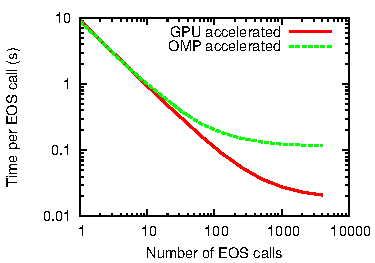
\includegraphics[width=0.5\linewidth]{eos_openacc.pdf}
%%   \begin{minipage}[b]{0.45\linewidth}
%%   \caption{Comparison of OpenACC (solid, red) and OpenMP (dashed,
%%     green) parallelizations of the EOS. Each calculation involves
%%     reading the EOS table into memory and then calling the EOS a
%%     certain number of times. The vertical axis shows the average time
%%     per call.  With few calls the execution time is dominated by
%%     reading the table into memory, but this is amortized out as we
%%     call the EOS more.  The OpenACC-threaded calls are significantly faster
%%     than the OpenMP-threaded calls, even when taking data movement to
%%     the GPU into account.\label{fig-eos-openacc}}
%%    \end{minipage}
%% \end{figure}

Our nuclear reaction integration is also being redesigned to target
GPUs.  For our XRB simulations, the reactions can represent a
significant fraction of the runtime (up to 25\% with our current,
small network).  Furthermore, we wish to use much larger networks to
better capture the nucleosynthesis and energetics of the burning.  To
facilitate this, we have added a new vectorized implicit ODE integrator to
\maestro\ written in modern Fortran
by our colleagues at LBNL.  We have successfully redesigned the integrator
to run entirely on accelerators using OpenACC.  An initial, unoptimized 
development version of a reactions unit test demonstrates a 2x speedup versus
perfect OpenMP scaling.  We have been working closely with OLCF to bring this
about and expect to be doing production science runs with GPU-accelerated
reactions by the time INCITE 2017 allocations begin.  \MarginPar{Bronson, Tom:
please review this paragraph}
In this proposal we expand
our collaboration to include scientists leading similar work on
offloading reactions to GPUs for other codes running
on titan (the Chimera core-collapse code~\cite{chimera-gpu} and the
S3D combustion code~\cite{s3d}).  By combining this expertise we will expedite
our acceleration efforts and design microphysics modules usable by a larger
suite of state-of-the-art reactive hydrodynamics codes. 

Finally we note that the porting of the microphysics to GPUs described
here applies to both \maestro\ and \castro, and furthermore, we will
make all of the resulting improvements available to the community.
Importantly, accelerated microphysics opens the door to new physics.
The network modifications will allow us to use larger, more realistic
reaction networks.  The GPU version of the EOS will allow us to 
``undo'' some of the common approximations used in hydrodynamics 
codes to avoid expensive EOS calls~\cite{colellaglaz:1985}, and improve our thermodynamic
consistency.

\MarginPar{Add discussion of multifab colors for MGFLD}

Scaling \boxlib's geometric multigrid (GMG) algorithms on GPUs is a high
priority for both \castro\ and \maestro. The massive parallelism on GPUs
amplifies the scalability challenges which GMG algorithms already face on
current multi-core architectures, particularly with regard to load imbalance at
coarse levels of the multigrid hierarchy. Happily, our integration of the
emerging benchmark GMG code HPGMG\footnote{\url{https://hpgmg.org/}} as an
external solver for \boxlib\ has provided a possible solution to this problem.
Recently, NVIDIA ported HPGMG to
CUDA\footnote{\url{https://devblogs.nvidia.com/parallelforall/high-performance-geometric-multi-grid-gpu-acceleration/}},
exploiting the Unified Memory feature introduced in CUDA 6, which simplifies
data synchronization between host and GPU memory. They pursued a ``hybrid''
implementation, in which relaxations at coarse levels with small grids execute
on the CPU, while those at the fine levels with large grids execute on the GPU.
By tuning the CPU-GPU grid size threshold, they achieved speedups of 400\% over
the pure-CPU version of HPGMG.

We will leverage this knowledge to explore similar implementations in \boxlib.
Although \boxlib's solvers are more general-purpose than HPGMG (e.g., they
support mixed boundary conditions, refined meshes, arbitrarily shaped
rectangular grids, cell-centered and nodal meshes, etc.), the heart of NVIDIA's
hybrid approach to GPU acceleration would benefit our in-house solvers as well.

A major goal of the united effort represented by this INCITE proposal \MarginPar{new}
is to create a single set of microphysics solvers (burners and EOSes)
that can be used by all codes.  We will combine our GPU optimizations
into a single suite that is made publicly available through a github
repo (tentatively called \starkiller).
